\begin{center}
\Huge
Punkter, vektorer og prikprodukt
\end{center}

\section*{Vektorer mellem punkter}
\stepcounter{section}
Har vi to punkter $A(a_1,a_2)$ og $B(b_1,b_2)$, så betegner vi vektoren mellem punkterne som
\begin{align*}
\vv{AB}.
\end{align*}
Vi kalder denne vektor for \textit{forbindelsesvektoren} fra $A$ til $B$.
Vi definerer derfor koordinaterne til vektoren $\vv{AB}$ ved 
\begin{align*}
	\vv{AB} = 
	\begin{pmatrix}
		b_1 - a_1\\b_2-a_2
	\end{pmatrix}.
\end{align*}
Som et vigtigt eksempel har vi vektoren fra punktet origo $O(0,0)$ til et punkt $P(p_1,p_2)$, der betegnes 
\begin{align*}
\vv{OP},
\end{align*}
og kaldes for \textit{stedvektoren} for $P$. 
Koordinaterne til vektoren $\vv{OP}$ er givet ved 
\begin{align*}
	\vv{OP} = 
	\begin{pmatrix}
		p_1\\p_2
	\end{pmatrix}.
\end{align*}
\begin{exa}
Stedvektoren til punktet $P(2,3)$ er givet ved 
\begin{align*}
	\vv{OP} = 
	\begin{pmatrix}
		2\\3
	\end{pmatrix}.
\end{align*}
Har vi også punktet $Q(-3,5)$, så er vektoren $\vv{PQ}$ givet ved
\begin{align*}
	\vv{PQ} =
	\begin{pmatrix}
		-3-2\\
		5-3
	\end{pmatrix} =
	\begin{pmatrix}
		-5\\2
	\end{pmatrix}.
\end{align*}
\end{exa}

\newpage
\section*{Længde af vektor}

Vi ønsker at definere længden af en vektor. 
\begin{defn}[Længden af en vektor]
	Længden af en vektor $\vv{v}$ med koordinaterne
	\begin{align*}
		\vv{v} = 
		\begin{pmatrix}
			v_1 \\ v_2
		\end{pmatrix}
	\end{align*}
	defineres som
	\begin{align*}
		|\vv{v}| = \sqrt{v_1^2 + v_2^2}.
	\end{align*}
\end{defn}
Den opmærksomme læser vil nok bemærke længdeformlens lighed med Pythagoras' sætning. 

\begin{exa}
	Vektoren $\vv{v}$ givet ved
	\begin{align*}
		\vv{v} = 
		\begin{pmatrix}
			-6 \\ 8
		\end{pmatrix}
	\end{align*}
	har længden 
	\begin{align*}
		|\vv{v}| = \sqrt{(-6)^2+8^2} = \sqrt{36+64} = \sqrt{100} = 10
	\end{align*}
\end{exa}

\begin{setn}[Afstand mellem to punkter]
Skal vi bestemme afstanden mellem et punkt $P(p_1,p_2)$ og et punkt $Q(q_1,q_2)$, så er det givet ved
\begin{align*}
\texttt{dist}(P,Q) = |\vv{PQ}| = \sqrt{(p_1-q_1)^2+(p_2-q_2)^2}
\end{align*}
\end{setn}
\begin{proof}
Vektoren $\vv{PQ}$ er givet ved
\begin{align*}
\vv{PQ}=\begin{pmatrix}
q_1-p_1\\q_2-p_2
\end{pmatrix}.
\end{align*}
Vi anvender nu blot formlen for længden af en vektor og får
\begin{align*}
|\vv{PQ}| = \sqrt{(q_1-p_1)^2+(q_2-p_2)^2}
\end{align*}
\end{proof}
\begin{exa}
Afstanden fra punktet $P(0,1)$ og punktet $Q(-1,2)$ er givet ved
\begin{align*}
\texttt{dist}(P,Q) = \sqrt{(-1-1)^2+(2-1)^2} = \sqrt{5}.
\end{align*}
\end{exa}

\newpage

\section*{Prikprodukt}
\stepcounter{section}

Vi vil ikke definere nogen måde at gange vektorer sammen. Vi vil i stedet definere det såkaldte prikprodukt. Dette kan blandt andet bruges til at bestemme vinklen mellem to vektorer. 
\begin{defn}
Lad $\vv{v}$ og $\vv{w}$ være defineret som
\begin{align*}
\vv{v} = \begin{pmatrix}
v_1\\ v_2
\end{pmatrix}, \textnormal{ og }\vv{w} = \begin{pmatrix}w_1 \\ w_2
\end{pmatrix}.
\end{align*}
Så defineres \textit{prikproduktet} eller \textit{skalarproduktet} mellem $\vv{v}$ og $\vv{w}$ som
\begin{align*}
v\cdot w = v_1w_1 + v_2w_2.
\end{align*}
Dette skrives også til tider $\langle \vv{v}, \vv{w} \rangle$. 
\end{defn}
\begin{exa}
Lad $\vv{v} = \begin{pmatrix}
2 \\ 2
\end{pmatrix}$ og lad $\vv{w} = \begin{pmatrix}
-2 \\ 5
\end{pmatrix}$. Så kan vi bestemme prikproduktet mellem $\vv{v}$ og $\vv{w}$ som
\begin{align*}
\vv{v} \cdot \vv{w} = 2\cdot(-2)+2\cdot 5 = 6.
\end{align*}
\end{exa}

\section*{Vinkler mellem vektorer}
\stepcounter{section}

Prikproduktet relaterer sig til vinklen mellem vektorer. Vi skal senere se, hvordan vi kan bestemme vinklen mellem to vektorer. Vinklen mellem to vektorer $\vv{v}$ og $\vv{w}$ noteres som $\angle(\vv{v},\vv{w})$. På Figur \ref{fig:vinkel} er vinklen mellem to vektorer illustreret
\begin{figure}[H]
	\centering
	\begin{tikzpicture}
		\begin{axis}[
			axis lines = center, 
			xmin = -1, xmax = 5, 
			ymin = -1, ymax = 5, 
			x = 1.5cm, y = 1.5cm,
			ticks = none, 
			xlabel = $x$, ylabel = $y$
		]
			\draw[-{Stealth[scale=1.5]}, thick, color = teal] (axis cs: 1,1) -- (axis cs: 3,4);
			\draw[-{Stealth[scale=1.5]}, thick, color = teal] (axis cs: 1,1) -- (axis cs: 4,0);
			\draw[thick,teal] ([shift=(-18.43:0.7cm)] axis cs: 1,1) arc (-18.43:56.31:0.7cm);
			\node[color = teal] at (axis cs: 1.6,1.2) {$\theta$};
			\node[color = teal] at (axis cs: 2.5,0.7) {$\vv{v}$};
			\node[color = teal] at (axis cs: 1.7,2.5) {$\vv{w}$};			
		\end{axis}
	\end{tikzpicture}
	\caption{Vinkel mellem to vektorer}
	\label{fig:vinkel}
\end{figure}

Hvis vinklen mellem to vektorer $\vv{v}$ og $\vv{w}$ er $90^\circ$, altså at 
$\angle(\vv{v},\vv{w}) = 90^\circ$, så siger vi, at vektorerne er vinkelrette eller \textit{orthogonale}. Vi skriver da $\vv{w} \perp \vv{v}$.

\begin{setn}\label{setn:1}
To vektorer $\vv{v}$ og $\vv{w}$ er orthogonale hvis og kun hvis $\vv{v}\cdot \vv{w} = 0$.
\end{setn}
Vi vil senere se mere præcist hvordan sammenhængen mellem vinklen mellem vektorer og prikproduktet er. 
\begin{exa}
Vi vil afgøre, om $\vv{v} = \begin{pmatrix}
2\\2
\end{pmatrix}$ og $\vv{w} = \begin{pmatrix}
-1\\1
\end{pmatrix}$ er orthogonale. Vi bestemmer derfor prikproduktet
\begin{align*}
\vv{v}\cdot \vv{w} = 2\cdot(-1)+2\cdot 1 = 0. 
\end{align*}
Derfor ved vi, at vinklen mellem de to vektorer er $0^\circ$, og at de derfor er orthogonale eller vinkelrette.
\end{exa}



\subsection*{Opgave 1}
	\begin{figure}[H]
		\centering
		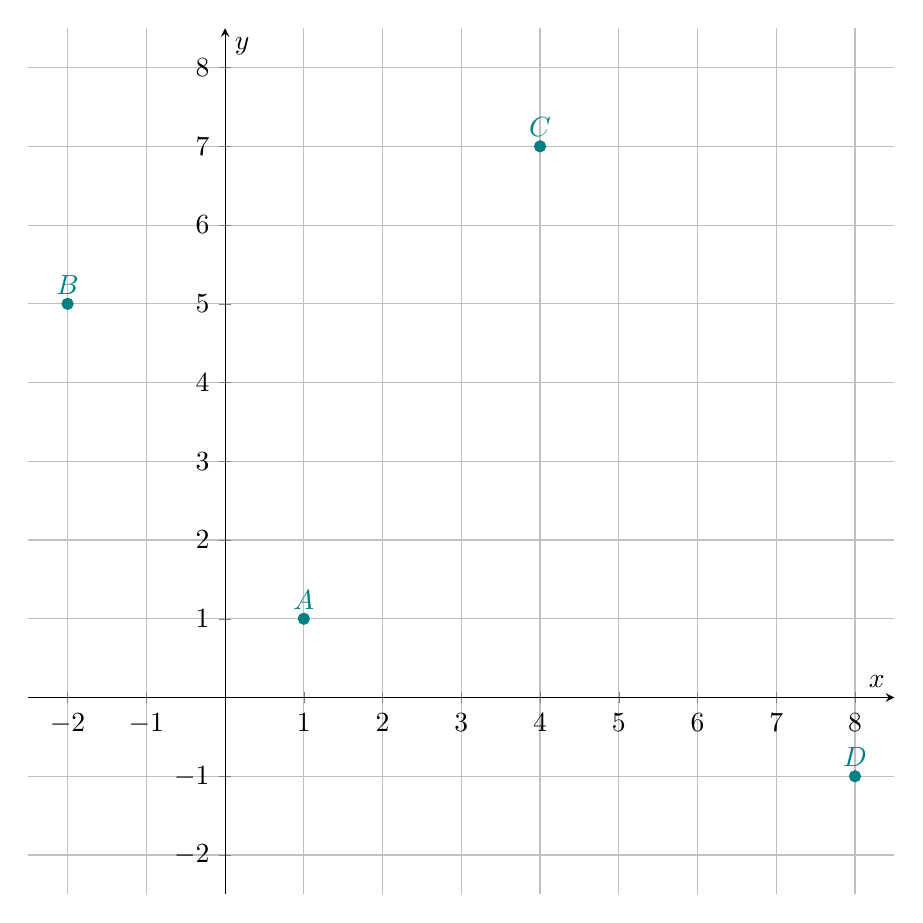
\begin{tikzpicture}
			\begin{axis}[
				axis lines = middle, 
				xmin = -2.5, xmax = 8.5,
				ymin = -2.5, ymax = 8.5,
				x = 1cm, y = 1cm,
				grid,
				xlabel = $x$, ylabel = $y$
			]
			\filldraw[teal] (axis cs: 1,1) circle (2pt) node[above] {$A$};
			\filldraw[teal] (axis cs: -2,5) circle (2pt) node[above] {$B$};
			\filldraw[teal] (axis cs: 4,7) circle (2pt) node[above] {$C$};
			\filldraw[teal] (axis cs: 8,-1) circle (2pt) node[above] {$D$};
			\end{axis}
		\end{tikzpicture}
		\caption{Repræsentanter for to vektorer}
		\label{fig:tovektorer}
	\end{figure}
\begin{enumerate}[label = \roman*)]
	\item Bestem koordinaterne for punkterne $A$, $B$ $C$ og $D$.
	\item Bestem koordinaterne til vektorerne $\vv{AB}$, $\vv{BC}$, $\vv{DA}$ og $\vv{BD}$.
	\item Bestem længden af vektorerne $\vv{AB}$, $\vv{BC}$, $\vv{DA}$ og $\vv{BD}$.
\end{enumerate}

\subsection*{Opgave 2}
\begin{enumerate}[label = \roman*)]
	\item For punkterne $A(2,5)$ og $B(4,9)$ kan du så uden at tegne punkterne gennemskue hvad
	koordinaterne til forbindelsesvektoren $\vv{AB}$ bliver?
	\item Hvis vi har to punkter $A(a_1,a_2)$ og $B(b_1,b_2)$, kan du så gennemskue, hvordan vi
	udregner koordinaterne til forbindelsesvektoren $\vv{AB}$?
\end{enumerate}


\subsection*{Opgave 3}

Bestem koordinaterne til stedvektoren til følgende punkter 
\begin{align*}
&1) \ (1,2)   &&2) \  (3,-1)  \\
&3) \  (\sqrt{2},\sqrt{5})  &&4) \ (-2,7)    \\
\end{align*}


\subsection*{Opgave 4}
Fire punkter er givet ved $A(1,3)$, $B(-5,6)$, $C(-4,1)$ og $D(12,-7)$.
\begin{enumerate}[label = \roman*)]
	\item Bestem koordinaterne til vektorerne $\vv{AB}$, $\vv{BC}$ og $\vv{DA}$.
	\item Bestem længden af vektorerne $\vv{AB}$, $\vv{BC}$ og $\vv{DA}$
	\item Bestem $\vv{BA} + \vv{CD}$.
	\item Bestem $|2\vv{CA} - 3\vv{BC} + \vv{DB}|$.
\end{enumerate}

\subsection*{Opgave 5}
Bestem afstanden mellem punkterne $A(6,3)$ og $B(9,7)$.


\subsection*{Opgave 6}
\begin{enumerate}[label=\roman*)]
\item Bestem prikproduktet mellem følgende vektorer
\begin{align*}
&1) \ \begin{pmatrix}1 \\ 0\end{pmatrix} \textnormal{ og } \begin{pmatrix}0 \\ 1\end{pmatrix}    &&2) \  \begin{pmatrix} 4 \\  5\end{pmatrix} \textnormal{ og } \begin{pmatrix} -2  \\ 6\end{pmatrix}    \\
&3) \ \begin{pmatrix}12 \\ 15\end{pmatrix} \textnormal{ og } \begin{pmatrix}-3 \\ 14 \end{pmatrix}   &&4) \ \begin{pmatrix} -2 \\ -5\end{pmatrix} \textnormal{ og } \begin{pmatrix} 0.5 \\ -12 \end{pmatrix}     \\
\end{align*}
\end{enumerate}

\subsection*{Opgave 7}

Afgør hvilke af følgende par af vektorer, der er orthogonale

\begin{align*}
	&1) \ \begin{pmatrix}
		2 \\ 5
	\end{pmatrix} 
	\textnormal{ og }
	\begin{pmatrix}
		-10 \\ 4
	\end{pmatrix} 
	&
	&2) \ \begin{pmatrix}
		4 \\ 11
	\end{pmatrix} 
	\textnormal{ og }
	\begin{pmatrix}
		-12 \\ 3
	\end{pmatrix} 
	\\
	&3) \ \begin{pmatrix}
		-0.5 \\ 3
	\end{pmatrix} 
	\textnormal{ og }
	\begin{pmatrix}
		12 \\ 0
	\end{pmatrix} 
	&
	&4) \ \begin{pmatrix}
		\frac{1}{4} \\ -8
	\end{pmatrix} 
	\textnormal{ og }
	\begin{pmatrix}
		16 \\ \frac{1}{2}
	\end{pmatrix} 
\end{align*}

\subsection*{Opgave 8}
Bestem prikproduktet mellem følgende vektorer.
\begin{center}
\resizebox{0.45\textwidth}{!}{
\begin{tikzpicture}
	\begin{axis}[
		axis lines = center, 
		xmin = -1.5, xmax = 6.5, 
		ymin = -1.5, ymax = 6.5,
		grid,
		x = 1cm, y = 1cm,
		xtick = {-1,0,...,5,6}, ytick = {-1,0,...,5,6},
		xlabel = $x$, ylabel = $y$	
	]
		\draw[-{Stealth[scale=1.5]}, thick, color = teal] (axis cs: 0,0) -- (axis cs: 4,5);
		\draw[-{Stealth[scale=1.5]}, thick, color = teal] (axis cs: 1,5) -- (axis cs: -1,-1);
	\end{axis}
\end{tikzpicture}
}
\resizebox{0.45\textwidth}{!}{
\begin{tikzpicture}
	\begin{axis}[
		axis lines = center, 
		xmin = -1.5, xmax = 6.5, 
		ymin = -1.5, ymax = 6.5,
		grid,
		x = 1cm, y = 1cm,
		xtick = {-1,0,...,5,6}, ytick = {-1,0,...,5,6},
		xlabel = $x$, ylabel = $y$	
	]
		\draw[-{Stealth[scale=1.5]}, thick, color = teal] (axis cs: 1,1) -- (axis cs: 6,-1);
		\draw[-{Stealth[scale=1.5]}, thick, color = teal] (axis cs: 1,1) -- (axis cs: 3,6);
	\end{axis}
\end{tikzpicture}
}
\end{center}

\subsection*{Opgave 9}
Afgør hvilke af følgende par af vektorer, der er orthogonale

\begin{center}
\resizebox{0.45\textwidth}{!}{
\begin{tikzpicture}
	\begin{axis}[
		axis lines = center, 
		xmin = -4.5, xmax = 2.5, 
		ymin = -4.5, ymax = 2.5,
		grid,
		x = 1cm, y = 1cm,
		xtick = {-4,-3,...,2,3}, ytick = {-4,-3,...,2,3},
		xlabel = $x$, ylabel = $y$	
	]
		\draw[-{Stealth[scale=1.5]}, thick, color = teal] (axis cs: -3,-2) -- (axis cs: 2,-4);
		\draw[-{Stealth[scale=1.5]}, thick, color = teal] (axis cs: -2,2) -- (axis cs: -4,-4);
	\end{axis}
\end{tikzpicture}
}
\resizebox{0.45\textwidth}{!}{
\begin{tikzpicture}
	\begin{axis}[
		axis lines = center, 
		xmin = -1.5, xmax = 6.5, 
		ymin = -1.5, ymax = 6.5,
		grid,
		x = 1cm, y = 1cm,
		xtick = {-1,0,...,5,6}, ytick = {-1,0,...,5,6},
		xlabel = $x$, ylabel = $y$	
	]
		\draw[-{Stealth[scale=1.5]}, thick, color = teal] (axis cs: 4,4) -- (axis cs: 6,6);
		\draw[-{Stealth[scale=1.5]}, thick, color = teal] (axis cs: 5,0) -- (axis cs: 0,5);
	\end{axis}
\end{tikzpicture}
}

\end{center}

\subsection*{Opgave 10}

Fire punkter er givet ved $A(2,2)$, $B(5,4)$, $C(-2,7)$ og $D(-7,-3)$.
\begin{enumerate}[label=\roman*)]
	\item Bestem $\vv{AB}\cdot \vv{CD}$
	\item Afgør om $\vv{AC}$ og $\vv{DB}$ er orthogonale
\end{enumerate}

\subsection*{Opgave 11}

To vektorer er givet ved
\begin{align*}
	\vv{a} = 
	\begin{pmatrix}
		x^2 - 2 \\
		1	
	\end{pmatrix}
	\textnormal{ og }
	\vv{b} = 
	\begin{pmatrix}
		1 \\
		x
	\end{pmatrix}
\end{align*}
\begin{enumerate}[label = \roman*)]
	\item Bestem $x$, så $\vv{a}$ og $\vv{b}$ er orthogonale.
\end{enumerate}
